%%%%%%%%%%%%%%%%%%%%%%%%%%%%%%%%%%%%%%%%%%%%%%%%%%%
%% LaTeX book template                           %%
%% Author:  Amber Jain (http://amberj.devio.us/) %%
%% License: ISC license                          %%
%%%%%%%%%%%%%%%%%%%%%%%%%%%%%%%%%%%%%%%%%%%%%%%%%%%

\documentclass[a4paper,11pt, oneside]{book}
\usepackage[T1]{fontenc}
\usepackage[utf8]{inputenc}
\usepackage{lmodern}
\usepackage{mathptmx}

% Uncomment to set page margin to 2.5 cm.
%\usepackage[margin=2.5cm]{geometry}

%%%%%%%%%%%%%%%%%%%%%%%%%%%%%%%%%%%%%%%%%%%%%%%%%%%%%%%%%
% Source: http://en.wikibooks.org/wiki/LaTeX/Hyperlinks %
%%%%%%%%%%%%%%%%%%%%%%%%%%%%%%%%%%%%%%%%%%%%%%%%%%%%%%%%%
\usepackage{hyperref}
\usepackage{graphicx}
\usepackage[english]{babel}
\usepackage{verbatimbox}
\usepackage{graphicx}
\graphicspath{ {schedule/}{diagrams/} }
\usepackage{float}
\usepackage{pdfpages}

%%%%%%%%%%%%%%%%%%%%%%%%%%%%%%%%%%%%%%%%%%%%%%%%%%%%%%%%%%%%%%%%%%%%%%%%%%%%%%%%
% 'dedication' environment: To add a dedication paragraph at the start of book %
% Source: http://www.tug.org/pipermail/texhax/2010-June/015184.html            %
%%%%%%%%%%%%%%%%%%%%%%%%%%%%%%%%%%%%%%%%%%%%%%%%%%%%%%%%%%%%%%%%%%%%%%%%%%%%%%%%
\newenvironment{dedication}
{
   \cleardoublepage
   \thispagestyle{empty}
   \vspace*{\stretch{1}}
   \hfill\begin{minipage}[t]{0.66\textwidth}
   \raggedright
}
{
   \end{minipage}
   \vspace*{\stretch{3}}
   \clearpage
}

%%%%%%%%%%%%%%%%%%%%%%%%%%%%%%%%%%%%%%%%%%%%%%%%
% Chapter quote at the start of chapter        %
% Source: http://tex.stackexchange.com/a/53380 %
%%%%%%%%%%%%%%%%%%%%%%%%%%%%%%%%%%%%%%%%%%%%%%%%
\makeatletter
\renewcommand{\@chapapp}{}% Not necessary...
\newenvironment{chapquote}[2][2em]
  {\setlength{\@tempdima}{#1}%
   \def\chapquote@author{#2}%
   \parshape 1 \@tempdima \dimexpr\textwidth-2\@tempdima\relax%
   \itshape}
  {\par\normalfont\hfill--\ \chapquote@author\hspace*{\@tempdima}\par\bigskip}
\makeatother

%%%%%%%%%%%%%%%%%%%%%%%%%%%%%%%%%%%%%%%%%%%%%%%%%%%
% First page of book which contains 'stuff' like: %
%  - Book title, subtitle                         %
%  - Book author name                             %
%%%%%%%%%%%%%%%%%%%%%%%%%%%%%%%%%%%%%%%%%%%%%%%%%%%

% Book's title and subtitle
\title{\Huge \textbf{Road Surface Estimator} \\ \huge Final Report}
% Author
\author{
	\textsc{Thanakrit Lee}
	\\
	26529009
	\\
	tlee38@student.monash.edu
	\\
	Monash University
}

\begin{document}
	
\frontmatter
\maketitle

%%%%%%%%%%%%%%%%%%%%%%%%%%%%%%%%%%%%%%%%%%%%%%%%%%%%%%%%%%%%%%%%%%%%%%%%

\begin{center}
	\textbf{Abstract}
\end{center}
Abstract goes here. Less than 300 words.

Lorem ipsum dolor sit amet, consectetur adipiscing elit. Integer massa quam, sodales at sapien a, feugiat pretium arcu. Aliquam augue leo, viverra at scelerisque eu, auctor quis lorem. Sed leo mauris, ultricies sit amet nibh ut, cursus consequat tellus. Integer suscipit interdum nunc vel pretium. Curabitur suscipit, dolor sit amet sodales rutrum, justo leo auctor dui, quis placerat nisl sapien ut purus. Curabitur ut venenatis nulla. Nulla ipsum libero, pretium in enim sed, interdum viverra ante.

Cras quam ex, venenatis id urna in, tincidunt sollicitudin ex. Suspendisse congue justo scelerisque orci varius, et facilisis odio auctor. Curabitur facilisis, orci ac tempor tempus, magna elit eleifend augue, et interdum ipsum sem in risus. Donec ex augue, mollis at enim vel, semper finibus odio. Quisque vel odio vel sapien eleifend condimentum. Pellentesque sed neque viverra, faucibus lorem tristique, mattis sem. Quisque condimentum tortor libero, quis malesuada libero sodales non.

\begin{center}
	\textbf{Keywords}
\end{center}
\begin{center}
	Keyword1, Keyword2, Keyword3, Keyword4, Keyword5
\end{center}

\begin{center}
	\textbf{Word Count}
\end{center}
\begin{center}
	3000 etc.
\end{center}




%%%%%%%%%%%%%%%%%%%%%%%%%%%%%%%%%%%%%%%%%%%%%%%%%%%%%%%%%%%%%%%%%%%%%%%%
% Auto-generated table of contents, list of figures and list of tables %
%%%%%%%%%%%%%%%%%%%%%%%%%%%%%%%%%%%%%%%%%%%%%%%%%%%%%%%%%%%%%%%%%%%%%%%%
\tableofcontents

\mainmatter

%%%%%%%%%%%%%%%%%%%%%%%%%%%%%%%%%%%%%%%%%%%%%%%%%%%%%%%%%%%%%%%%%%%%%%%%

\chapter{Introduction}

Re-surfacing roads requires the knowledge of the surface area of roads to resurface.
Getting the surface area of roads can be made more efficient using aerial/satellite views technology, where the surface area can be calculated. The efficiency of having a total estimated surface area of roads to resurface allows road surface materials to be prepared in a more precise manner, reducing materials wastes and thus reducing total road resurfacing costs.

\section{Objective}

The objective of this application is to allow user to select a point on the map and to work out the total area of roads in the nominated square kilometre, where the specified point is the centre, to give a quote of the road resurfacing cost \cite{DOCUMENT_PROJECT_INTRO:1}.

This web application that allows user to designate point on a map for a total estimated surface area of roads in the square kilometre ($km^2$). The web application will be implemented with Google Maps, which allows for user-to-map interactivity, and for getting data requires for the surface area calculation.

\section{Requirements}

\subsection{Functional Requirements}

\begin{itemize}
	\item The application is able to display a graphical map.
	\item The application allow user to interact with the map e.g. click on the map, drag and move around on the map, zoom in and zoom out, change map styling (roadmap and satellite view), add marker, move marker by dragging it, click on marker to show marker info.
	\item The application allow user to mark the centre point of the square kilometre area on the interactive map.
	\item The application allow user to input longitude and latitude coordinates.
	\item The application is able to display the user input coordinates on the interactive map.
	\item The application is able to calculate the surface area of the road in the selected square kilometre ($km^2$).
	\item The application is able to display the calculated road surface area.
\end{itemize}

\subsection{Non-Functional Requirements}
\begin{itemize}
	\item The application's graphical user interface is easy to navigate.
	\item The application is doesn't take long to process the surface area calculation, i.e. low response time.
	\item The application is responsive.
	\item The application is able to be use on mobile devices.
	\item The application provides an easy to understand tutorial on how to use the application.
	\item The application is hosted on the web, and user can access via the internet.
\end{itemize}

\section{Constraints}

A constraint for the project is that this project is done as part of a contract for a local council in Victoria, Melbourne, Australia. This means that the roads to resurface must be the correct category of roads classified by the local council (i.e. the declared roads being free ways, arterial roads and some non-arterial state roads) \cite{WEBSITE_VICROAD:1}.


%%%%%%%%%%%%%%%%%%%%%%%%%%%%%%%%%%%%%%%%%%%%%%%%%%%%%%%%%%%%%%%%%%%%%%%%

\chapter{Background}

\section{Academic Literature Review}
\begin{itemize}
	\item FIT3036 Project Intro Document \cite{DOCUMENT_PROJECT_INTRO:1}.
	
	The document gives a brief introduction to what the project will be about and the main specifications for the project. This document was use as the main reference for getting the requirements for the project's application.
	
	
	\item The Google Maps JavaScript API Documentation \cite{WEBSITE_GOOGLE_MAPS:1}.
	
	The documentation pages was use to study the API and how to use it in the project. Google Maps API was chosen, because it was one of the recommended technologies to use in the project specified in the project intro document \cite{DOCUMENT_PROJECT_INTRO:1}.
	
	
	\item Road Detection Using Deep Neural Network In High Spatial Resolution Images \cite{ARTICLE_ROAD_DETECTION:1}.
	
	This was the first article I read about road detection. I initially had the idea that the road detection was going to be done using satellite images. This article provide me with an overall look idea of how road detection was done using satellite images and deep Convolutional Neural Network (CNN).
	
	Although in the end I didn't end up implementing the application using satellite images and neural network, this article gives me a perspective of the different ways the application could be implemented.
	
	
	\item A Medium \cite{WEBSITE_MEDIUM:1} article. Node.js get-pixels: Getting Pixels at Specific Sectors of an Image using ndarray \cite{WEBSITE_MEDIUM_NODEJS_GET-PIXELS:1}
	
	This Medium article is a tutorial describing the way to get each pixel of an image using Node.js \cite{WEBSITE_NODEJS:1} and the package: get-pixels \cite{WEBSITE_GET-PIXELS:1}. I use this article to understand how to get each pixel of the map image using get-pixels.
	
	The article was useful in that it is simple, to the point, and provide lots of usage examples, while the get-pixels documentation doesn't provide lots of example for me to understand its usage.
	
	I believe my lack of understanding using the get-pixels documentation was that it doesn't provide any examples for the image pixels data structure \cite{WEBSITE_NDARRAY:1}, while the Medium article does.
	
	
	\item Google Maps Static Api Documentation \cite{WEBSITE_GOOGLE_MAPS_STATIC:1}.
	
	This documentation was use to understand how to create a static image of Google map. The static image is needed so that it could be processed in the server to detect the road pixels. The documentation is simple to understand, since there isn't any new concept introduce. The map URL property is almost the same as the JavaScript API, but is converted into a static image instead.
	
	
	\item Angular 5 tutorial and documentation \cite{WEBSITE_ANGULAR:1}
	
	I've decided to use the Angular (5) framework, because I want to make my development process of the application easier. I've also decided to use Angular, because I've recently started learning the technology and wanted to implement my knowledge.
	
	The tutorial provide a basic concept and usage of the framework, but I've also use other sources such as YouTube videos and online tutorial.
	
	The documentation is easy to understand as long as one have a grasp of the previous pre-requisite concepts. 
	
	
	\item A YouTube video tutorial on Angular Google Maps (AGM). Google Maps \& Angular | ANGULAR SNIPPETS \cite{WEBSITE_YOUTUBE_AGM:1}.
	
	The video shows how to get AGM setup and goes through the basic usage of the package: showing the map on a html page, adding markers to the map, and centring the map on a latitude/longitude coordinates.
	
	
	\item A video and online tutorial on how to use material design \cite{WEBSITE_GOOGLE_MATERIAL_DESIGN:1} bootstrap \cite{WEBSITE_BOOTSTRAP:1} with angular by using the library MDBootstrap \cite{WEBSITE_MDBOOTSTRAP:1}. Material Design Bootstrap 4 and Angular 5 Tutorial - MdBootstrap \cite{WEBSITE_COURSETRO_MDBOOTSTRAP_ANGULAR:1}.
	
	
	\item Bootstrap 4 documentation \cite{WEBSITE_BOOTSTRAP:1}.
	
	The documentation is use for when I've encounter Bootstrap related problem and the MDBootstrap documentation isn't clear or have enough information.
	
	
	\item Google Maps APIs Styling Wizard \cite{WEBSITE_GOOGLE_MAPS_API_STYLING_WIZARD:1}.
	
	The styling wizard is a tool use for creating a style property of a Google Maps. The wizard shows options such as colours and visibility of elements on the map. I've used this styling wizard for creating an appropriate style for my map where the roads are shown clearly and everything else is transparent. This style allows my application to classify the road pixels more efficiently.
	
	\item Google Chrome DevTools \cite{WEBSITE_GOOGLE_CHROME_DEVTOOLS:1}.
	
	"Chrome DevTools is a set of web developer tools built directly into the Google Chrome browser. DevTools can help you diagnose problems quickly, which ultimately helps you build better websites, faster." \cite{WEBSITE_GOOGLE_CHROME_DEVTOOLS:1}. 
	
	I've use the tools for debugging my web application, and for testing the mobile view of the application.
	
	The debugging feature that I've mainly use is the console output. I've use the console to log variables in my application to see if they're the expected variables, and to read the error logs when my application is bugged.
	
	I've discovered the mobile view only recently and thought that it would help me develop my application better to also be use on the mobile platform. The mobile view shows the application running on mobile screen device. The application is compacted to fit the screen. There are various mobile devices to choose from such as the iPhones, iPad, Galaxy, Pixel etc.
	
	
\end{itemize}

\section{Research}

\begin{itemize}
	\item MEAN stack.
	
	During the 2017 December break I was studying the MEAN web application stack. "MEAN" stands for MongoDB ExpressJS Angular NodeJS. A "stack" is a set/combination technologies that are use to together to create a web application. MongoDB is use as the application database. ExpressJS via NodeJS is use as the API server to connect the client-to-server-to-database. Angular is use as the interface for the client-side.
	
	My understanding of how a web application connects with each other have given me insight into how to better develop a web application, with better structure and business logic.
	
	The MEAN stack have influenced me in choosing the technologies I have chosen for this project (Angular, NodeJS, ExpressJS).
	
\end{itemize}



\section{Datasets}

\section{Risks}

\addvbuffer[12pt 8pt]{
	\begin{tabular}{ |p{1cm}||p{6cm}|p{6cm}| }
		\hline
		\multicolumn{3}{|c|}{\textbf{Risk List}} \\
		\hline
		\textbf{ID} & \textbf{Risk} & \textbf{Trigger} \\
		\hline
		R0 	& 	Project scope creep 	&	 Project scope wasn't defined properly. \\
		\hline
		R1	&	Software libraries, modules or frameworks changes and is now incompatible with the project	&  The software developers making changes to the software. \\
		\hline
		R2	&	Working computer breaks		&	Dropping the computer, spilling water on it. \\
		\hline
		R3	&	Project going over schedule		&	Improper time management of the project, not regularly updating and checking on the project schedule Gantt Chart.s \\
		\hline
\end{tabular}}
\vspace{3mm}
\addvbuffer[12pt 8pt]{
	\begin{tabular}{ |p{1cm}||p{6cm}|p{6cm}| }
		\hline
		\multicolumn{3}{|c|}{\textbf{Risk List}} \\
		\hline
		\textbf{ID} & \textbf{Probability (low/medium/high)} & \textbf{Impact (low/medium/high)} \\
		\hline
		R0 & low & high \\
		\hline
		R1 & low & medium \\
		\hline
		R2 & low & high \\
		\hline
		R3 & medium & high \\
		\hline
\end{tabular}}
\vspace{3mm}
\addvbuffer[12pt 8pt]{
	\begin{tabular}{ |p{1cm}||p{12.43cm}| }
		\hline
		\multicolumn{2}{|c|}{\textbf{Risk List}} \\
		\hline
		\textbf{ID} & \textbf{Mitigation Plan} \\
		\hline
		R0 & Make sure to get most (if not all) the project requirements from the project stakeholders. If a compulsory requirement is added, make it a priority over lower priority requirements. \\
		\hline
		R1 & Use versioning tool to keep track of the version of the libaries the project is using. \\
		\hline
		R2 & Take good care of the computer. Backup the project code regularly. Use Git remote repository (such as GitHub\cite{WEBSITE_GITHUB:1}) to backup the project and regularly make commits and push to the remote repository. \\
		\hline
		R3 & Regularly check the project schedule to see where the project progress is at and compare it to the current time to see if the project is behind, ahead or on schedule. Make a commitment to at keep the project on schedule. If the project is behind schedule then work over time to catch up to the project schedule time line.  \\
		\hline
\end{tabular}}

The only risk that was actually encountered in the project was R0: Project scope creep. 
\\\\
During the project a new requirement was added. The requirement was to add a a function to the application that allow the user to change the view of the map from "normal" view to a view that only shows roads. This requirement was added to give user more interactivity with the map, which in turn increase user experience (UX). 
\\\\
This scope creep was obviously the result of not property defining all the requirements needed in the requirement gathering phase. The risk trigger hypothesised in the risk document (from the project proposal) \cite{DOCUMENT_PROJECT_PROPOSAL:1} prove to be correct.
\\\\
To mitigate for the risk was that I accepted the risk that a new requirement was added to the project, and I assign a priority level to the new requirement in comparison to other requirements. I then work on implementing the highest priority level requirement then moving on to the lower ones. I used the same risk mitigation method as described in the risk document.


\section{Resource Requirements}
\begin{itemize}
	\item Computer for developing the project.
	
	\item Internet access to download and use libraries the project depends on, and to access the libraries documentation.
	
	\item Angular 5.2.0\cite{WEBSITE_ANGULAR:1}, a front end framework use for creating a good user interface and implementing business logic.
	
	\item Node.js 8.9.4\cite{WEBSITE_NODEJS:1}, a JavaScript runtime for use with Express.js to create a server API and implement the back end of the web application.
	
	\item Express.js 4.16.3\cite{WEBSITE_EXPRESSJS:1}, for creating the API for communication between client and server.
	
	\item MDBootstrap 5.2.3\cite{WEBSITE_MDBOOTSTRAP:1}, use the CSS framework for faster development of the app.
	
	\item AGM 1.0.0\cite{WEBSITE_AGM:1}, a wrapper of Google Maps JavaScript API for Angular 2+.
	
	\item Google Maps JavaScript API \cite{WEBSITE_GOOGLE_MAPS:1}. The JavaScript API is use to display a Google map on the web application for user to interact with. 
	
	\item Google Maps Static API \cite{WEBSITE_GOOGLE_MAPS_STATIC:1}. The Static API is use to create a static image URL from the JavaScript API so that the image could be process to find the roads area.
	
	\item get-pixels \cite{WEBSITE_GET-PIXELS:1}. A NodeJS package that get all pixels from an image. I use this package to extract the pixels from the Google map static image for classifying the road pixels.
	
	\item Syntactically Awesome Style Sheets (SASS) \cite{WEBSITE_SASS:1}. A style sheet language that is use with MDBootstrap to style html pages.
	
	\item Microsoft Virtual Studio Code (VS Code) \cite{WEBSITE_MICROSOFT_VSCODE:1}. An open source code editor that I use to edit the web application code.
	
	\item Google Chrome \cite{WEBSITE_GOOGLE_CHROME:1}. A internet browser for testing the functionality and user interface of the application.
	
	\item Goole DevTools \cite{WEBSITE_GOOGLE_CHROME_DEVTOOLS:1}. I use the tools for debugging my application.
	
	\item Git \cite{WEBSITE_GIT:1}. A version control system (VCS) that I use to keep track of the versions of the application. A good practice for software development is to use VCS while developing the software. Using git it has allow me to easily revert my application back to the previous version, and to easily add in bug fixes into the application.
	
	\item GitHub \cite{WEBSITE_GITHUB:1}. A Git remote repository. I use GitHub to host my Git repository remotely on the GitHub server for backup. I want to have a remote backup repository to mitigate the risk that something might go wrong with the computer I'm working on.
	
	\item GitKraken \cite{WEBSITE_AXOSOFT_GITKRAKEN:1}. A Git Graphical User Interface (GUI). I use GitKraken to streamline the application development process so that I can develop the application faster.
	
	\item Heroku \cite{WEBSITE_HEROKU:1}. A cloud platform as a service (Paas) \cite{WEBSITE_WIKIPEDIA_PAAS:1} use as a web application deployment model. I use Heroku to host my web application.
\end{itemize}

\section{Project Tasks}

The tasks required to be done for the project are listed in the Gantt chart below.

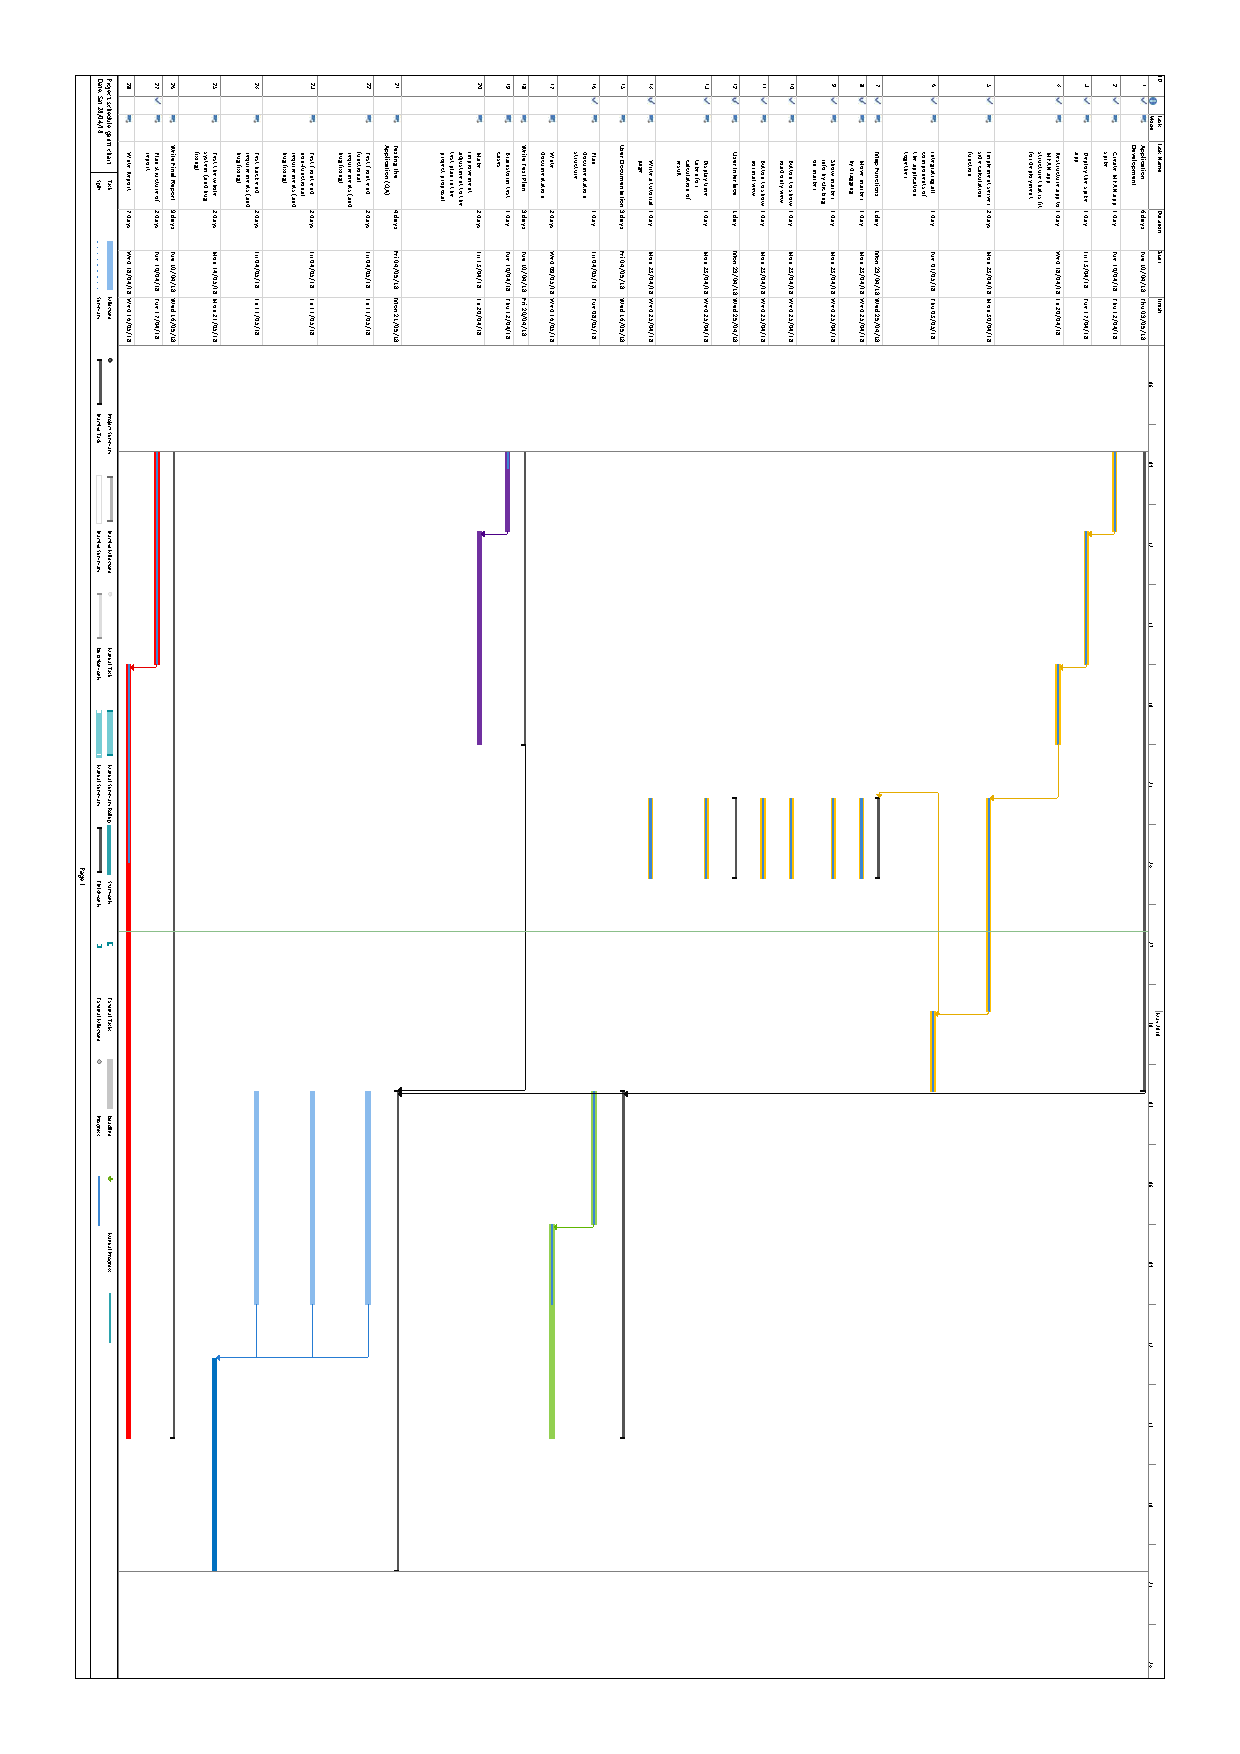
\includepdf[pages={1}]{schedule/schedule-gantt-chart-1-rotated.pdf}

As of writing the final report I'm behind schedule on my progress of the:
\begin{itemize}
	\item Final report.
	
	I'm currently behind my final report schedule progress by 2 days, but I'm expected catch up.
	
	\item Test plan
	
	I haven't started on rewriting my test plan from the project proposal yet. 
	
	\item Testing the application
	
	Although I haven't officially tested the application properly yet, I have had my application gone through usability tests and the result were good. I've also gotten criticism from the users and have made improvements to my application user interface to make my application more user friendly.
	
	\item Application documentations.
	
	I have only documented my application by 50\% so far.
	
\end{itemize}
My plan to get my project back on schedule is to first complete the final report, then complete the test report, test my application, and then document my application.
\\\\
I know that the project will be back in schedule in a week time.


%%%%%%%%%%%%%%%%%%%%%%%%%%%%%%%%%%%%%%%%%%%%%%%%%%%%%%%%%%%%%%%%%%%%%%%%

\chapter{Method}

I've used the Agile software development framework methodology in developing the project software product. For each sprint (week) I make small increments to the application. The increments are the functional and non-functional requirements. As I implement the requirements to the application I test each requirements to make sure that they are working as expected.
\\\\
The project schedule Gantt chart figure does not represent the Agile development life cycle I went through, but is a good basis as a list of tasks required for the project.

\section{Internal Design}

\section{Software Architecture}

\section{Algorithms}

In processing the map image to calculate the estimated total surface area of roads in a nominated square kilometre, I've use get-pixels (a NodeJS package) to extract all pixels from the map image.
\\\\
With all pixels from the map I run through all pixels from the top left corner of the map to the bottom right corner of the map once. While running through each pixel the pixel is check if it is visible or not, because only road pixels in the image are visible (this was done by styling the map using the styling wizard). If the pixel is visible, it is a road pixel and a counter is incremented by 1, if the pixel is not visible then do nothing. Once all pixels have been checked, the count of road pixels are multiplied by the square metre value of each pixel, given by the formula \cite{WEBSITE_GOOGLE_GROUPS_MAPS:1}	:
\begin{center}
	$squareMetrePerPixel = metresPerPixel \times metrePerPixel$
\end{center}

\begin{center}
	$metresPerPixel = \frac{156543.03392 \times \cos(lat \times \frac{\pi}{180})}{2^{zoom}}$ 
\end{center}
where
\begin{itemize}
	\item $lat$ is the latitude is the nominated square kilometre centre coordinates latitude.
	\item $zoom$ is the current zoom level of the map.
\end{itemize}
After the multiplication the result is the estimated total surface area of all roads in the nominated square kilometre in square metres. To convert to square kilometres divide the result by 1000000.

The activity diagram below shows the algorithm steps described above.

\begin{figure}[H]
	\begin{minipage}[b]{0.4\textwidth}
		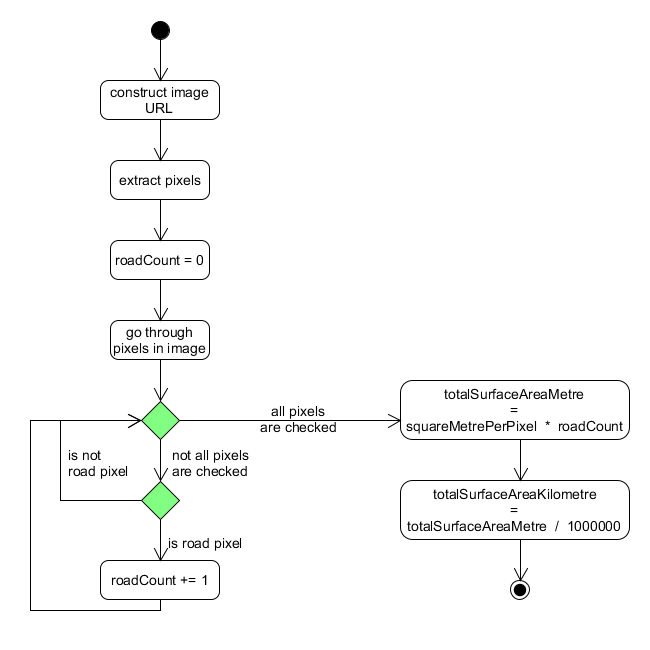
\includegraphics[scale=0.6]{algorithm.png}
		\caption{The total surface area calculation algorithm.}
	\end{minipage}
\end{figure}




%%%%%%%%%%%%%%%%%%%%%%%%%%%%%%%%%%%%%%%%%%%%%%%%%%%%%%%%%%%%%%%%%%%%%%%%

\chapter{Results}
% Analyse the OUTCOMES and QUALITY of the project.

\section{Externally Observable Features}

\section{Performance}


%%%%%%%%%%%%%%%%%%%%%%%%%%%%%%%%%%%%%%%%%%%%%%%%%%%%%%%%%%%%%%%%%%%%%%%%

\chapter{Analysis \& Discussion}
% Analyse the statics and outputs.

% If you don’t have any idea how this kind of research might be reported, look at a few research articles in the journal JASSS: http://jasss.soc.surrey.ac.uk/JASSS.html


%%%%%%%%%%%%%%%%%%%%%%%%%%%%%%%%%%%%%%%%%%%%%%%%%%%%%%%%%%%%%%%%%%%%%%%%

\chapter{Future Work}
% Include also any possible future research that might emanate from the project.


%%%%%%%%%%%%%%%%%%%%%%%%%%%%%%%%%%%%%%%%%%%%%%%%%%%%%%%%%%%%%%%%%%%%%%%%

\chapter{Conclusion}


%%%%%%%%%%%%%%%%%%%%%%%%%%%%%%%%%%%%%%%%%%%%%%%%%%%%%%%%%%%%%%%%%%%%%%%%

\chapter{References}
% Organise the bibliography alphabetically by first-author surname or by order of appearance in the article.

\bibliography{reference/reference}
\bibliographystyle{apalike}

%%%%%%%%%%%%%%%%%%%%%%%%%%%%%%%%%%%%%%%%%%%%%%%%%%%%%%%%%%%%%%%%%%%%%%%%

\chapter{Appendices}

\section{Production and Deployment}
% Detail instructios to run/install/compile your software, with complete instructions/screenshots. Include all information such as dependencies, platform, etc.

\section{Parameters}
% GUI, input, boxes, choicecs, etc.

\section{User Interface}
% How to run the software.
% Detail clearly the interface(s) to the Web-based project.

\section{Externally Available Functions}
% Debuggin tools, auxilliary/helper function, bonus features.

\section{Internal Testing Procedures}
% Cross-references to Test Report.

%%%%%%%%%%%%%%%%%%%%%%%%%%%%%%%%%%%%%%%%%%%%%%%%%%%%%%%%%%%%%%%%%%%%%%%%

\end{document}